\section{Teil \uproman{2}: Frank-Hertz-Versuch}

\subsection{Aufbau}
    \begin{itemize}
        \item Vorgehen beim Aufbau
        \item Bestimmung von $U\sub{1,max}$
    \end{itemize}

\subsection{Messung unter variabler Bremsspannung $U_2$}
    \begin{itemize}
        \item Spektrum mit Gauß fitten
        \item Maxima, Halbwertsbreiten und $\Delta U$ bestimmen
        \item Einfluss von $U_2$ diskutieren
    \end{itemize}
    
\subsection{Messung unter variabler Temperatur $T$}
    \begin{itemize}
        \item Spektrum mit Gauß fitten
        \item Maxima, Halbwertsbreiten und $\Delta U$ bestimmen
        \item Einfluss von $T$ diskutieren
    \end{itemize}

\subsection{Ergebnisse}
    \begin{itemize}
        \item $\Delta E$ Vergleich Literaturwert
        \item Einfluss Wirkungsquerschnitt diskutieren
        \item Warum keine scharfen Einbrüche in Anodenstrom?
        \item Warum kleines Temperaturintervall bei Hg?
        \item Zusammenhang mit konkreten Hg-Übergängen
        \item Zusammenhang von Hg-Gasdruck und Temperatur
    \end{itemize}


    \begin{figure}[H]
        \centering
        \begin{subfigure}{0.4\textwidth}
            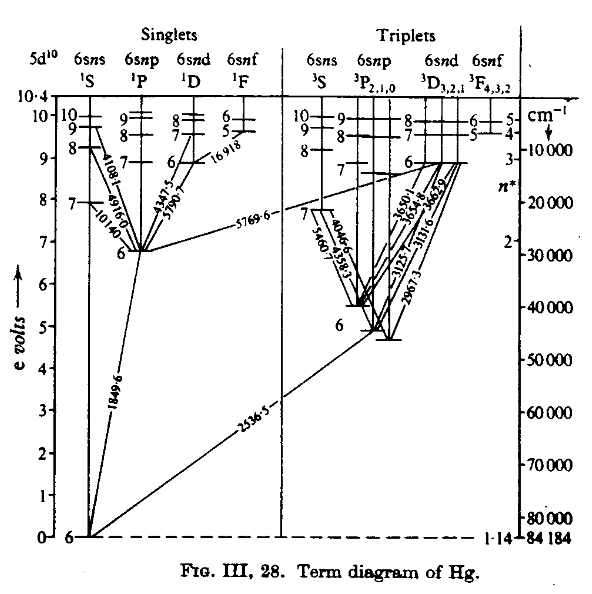
\includegraphics[width=\linewidth]{figs/Hertz_Termdiagramm_Hg.png}
            \caption{Vereinfachtes Hg-Termschema. \cite{Hertz_Termschema_Hg-Abb}}
        \end{subfigure}
        \hspace{1cm}
        \begin{subfigure}{0.45\textwidth}
            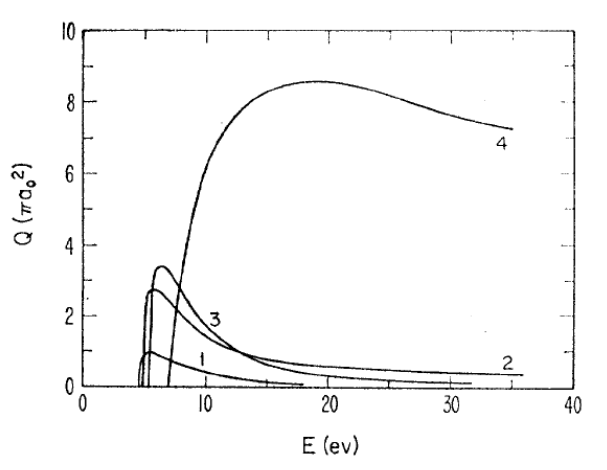
\includegraphics[width=\linewidth]{figs/Hertz_Wirkungsquerschnitte.png}
            \caption{Totaler Wirkungsquerschnitt von Hg für Elektronenstoßanregung. \cite{Hertz_Wirkungsquerschnitt-Abb}}
        \end{subfigure}
        \caption{}
    \end{figure}